\chapter{Antenna Data Characteristics}
\label{chap:antenna}
\begin{strip}
	\begin{minipage}{\textwidth}
		\begin{abstract}
			In this chapter I study the effect that antenna type has on the data produced by said antenna. This is done through an analysis of key characteristics describing important qualities of the data at hand. I find that, though there is variation between the differing types, there is no clear advantage for any of the considered antenna types. However, I also find that there are some indications as to which antenna type receives the best detection counts which may influence which antennas are used for future radio detection stations.
		\end{abstract}
	\end{minipage}
\end{strip}
\section{Background}
Radio meteor detection can use a variety of different antenna types. There are 12 main types used in the RMOB data I am using. Yagi antennas are overwhelmingly the most popular, followed by dipole antennas (see figure~\ref{fig:antennas}).
\begin{figure}[h!]
	\centering
	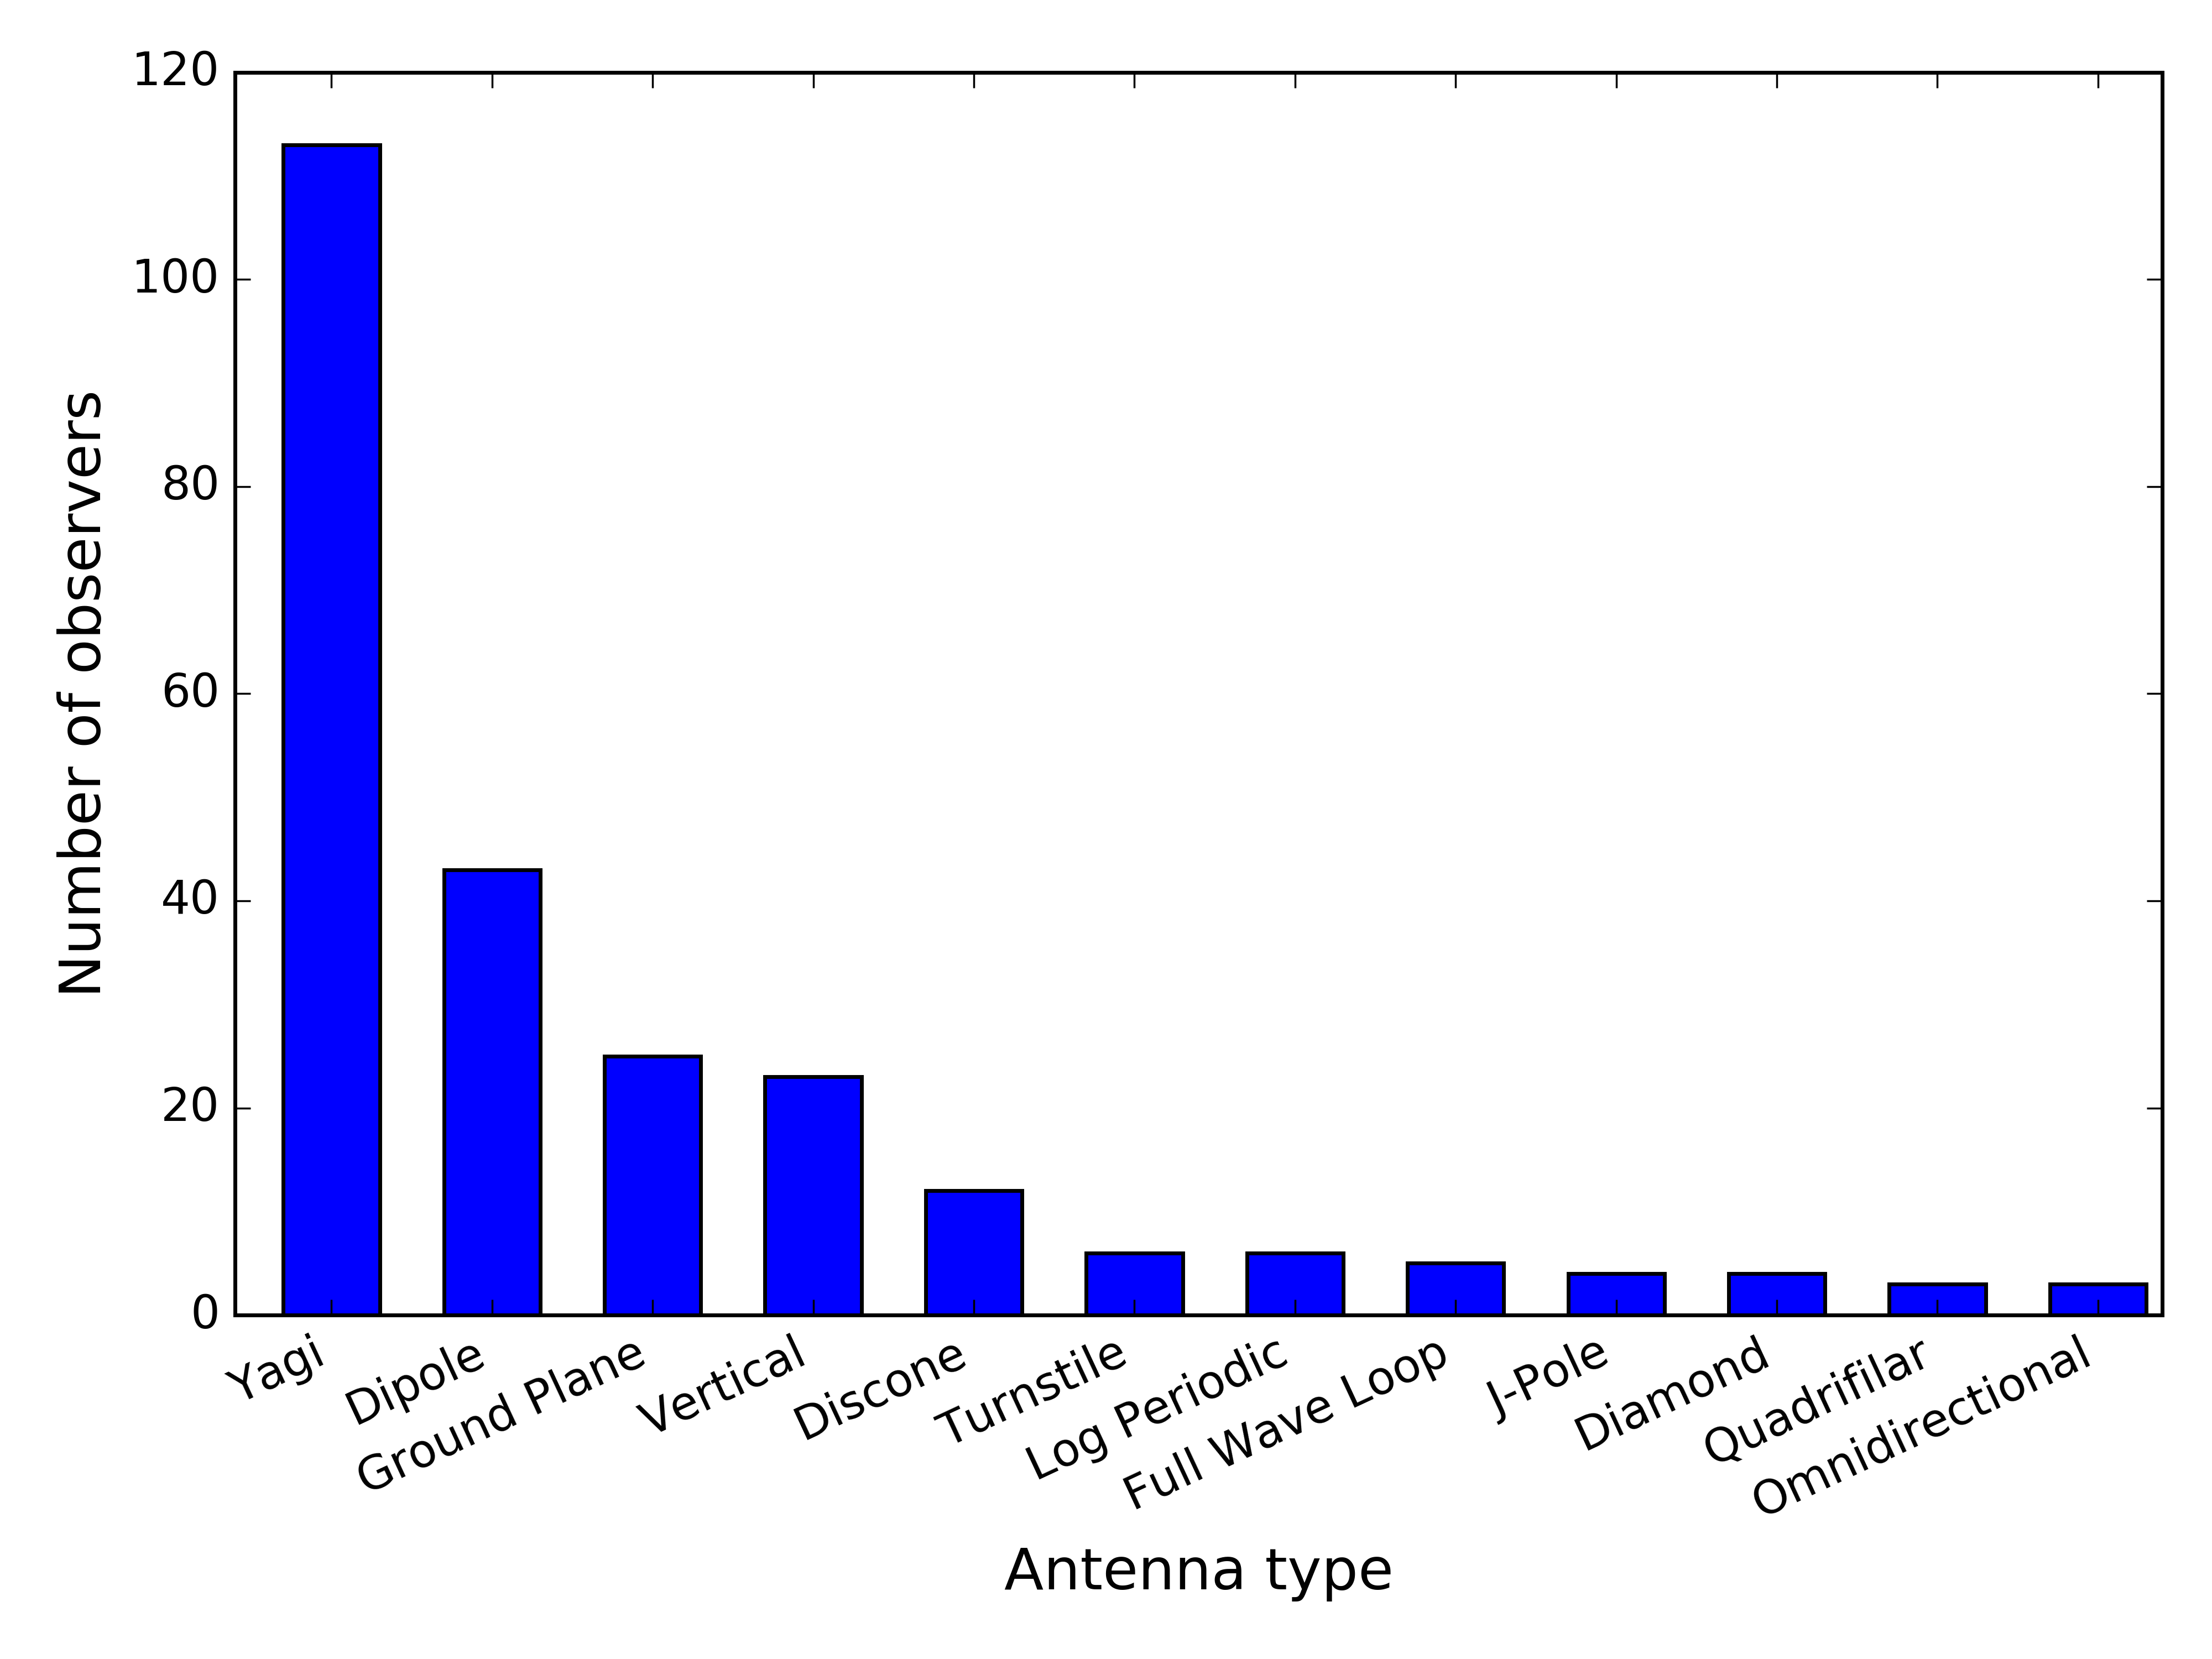
\includegraphics[width=\linewidth]{antennas}
	\caption{Antenna usage in RMOB data \label{fig:antennas}}
\end{figure}
Each antenna type has its own merits and cons, but that is a a discussion for another report. 
\section{Methodology}
\subsection{Selecting authors}
There are 12 antenna types that will be analysed. In order to carry out the analysis, the observers must be split into groups for each of these types. This was done through manual selection: displaying the antenna type of each observer (if it has one), and choosing which type this antenna is, through a Python program. Any unknown types were declared as miscellaneous. These categories were then saved to their own file.
\subsection{Analyses}
The analysis focused on 6 values, aimed at summarising and describing the detections made by the observers in each antenna category. Two of these values are the mean and maximum of all data collected by each respective observer. The minimum is of little importance, since the value will almost always be 0 or 1. These indicate the typical detection counts for the observer. The standard error of the same data set is also taken, which indicates how much the data varies. A lower value indicates that the same detection count is generally seen, and a larger value indicates that the detection count varies erratically. The skew also indicates the distribution of the detection counts. A positive skew indicates that the detection counts trail off towards high values, whilst a negative skew indicates that the distribution is `steeper' for higher values, suggesting that there is a limit to the detection counts. The last two values are the peak hour of the diurnal shift, and the fit to an optimised sine curve for the mean detection counts over each hour of a day. This is calculated by averaging the values for all data for a given hour after midnight. A sine curve is in then fit to this, in the same process as chapter~\ref{chap:diurnalshift}, giving a sine function of the form $N = A \sin \left( \omega t + \phi \right) + \mu$ where $N$ is the detection count and $t$ is the hour. The calculated `fit' is the sum of the standard deviations for $A$, $\mu$, and $\phi$. $\omega$ is assumed to be $\frac{2\pi}{24}$ so that the shift has a period of one day. A comparison is made of these 6 values for each antenna type.
\subsection{Sample sizes}
Sample sizes for each antenna category are shown below.
\begin{table}[h!]
	\begin{tabular}{cc}
		\hline
		Antenna & N$^o$ observers \\ \hline
		Diamond & 4 \\
		Discone & 12 \\
		Full wave loop & 5 \\
		Ground plane & 25 \\
		J-pole & 4 \\
		Log periodic & 6 \\
		Omni & 3 \\
		Quad & 3 \\
		Turnstile & 6 \\
		Vertical & 23 \\
		Yagi & 113 \\
		\hline
	\end{tabular}
\end{table}

\section{Results}
\subsection{Mean \& maximum}
Figure~\ref{fig:ant:meanmaxmin} shows the result for the mean and maximum counts for each hour, averaged for each respective antenna type. There is no clear difference between the means, as shown by the error bars, which show standard error. The largest mean is for a Turnstile antenna, though this is likely due to a single observer with a large detection count, and this is supported by the large standard error. There is also no significant difference in the maximum values. The most extreme (both large and small) maximum counts have larger error bars, which suggests that there are only a few observers which have these maximum counts out of all those in the antenna category.

\begin{figure}[h!]
	\centering
	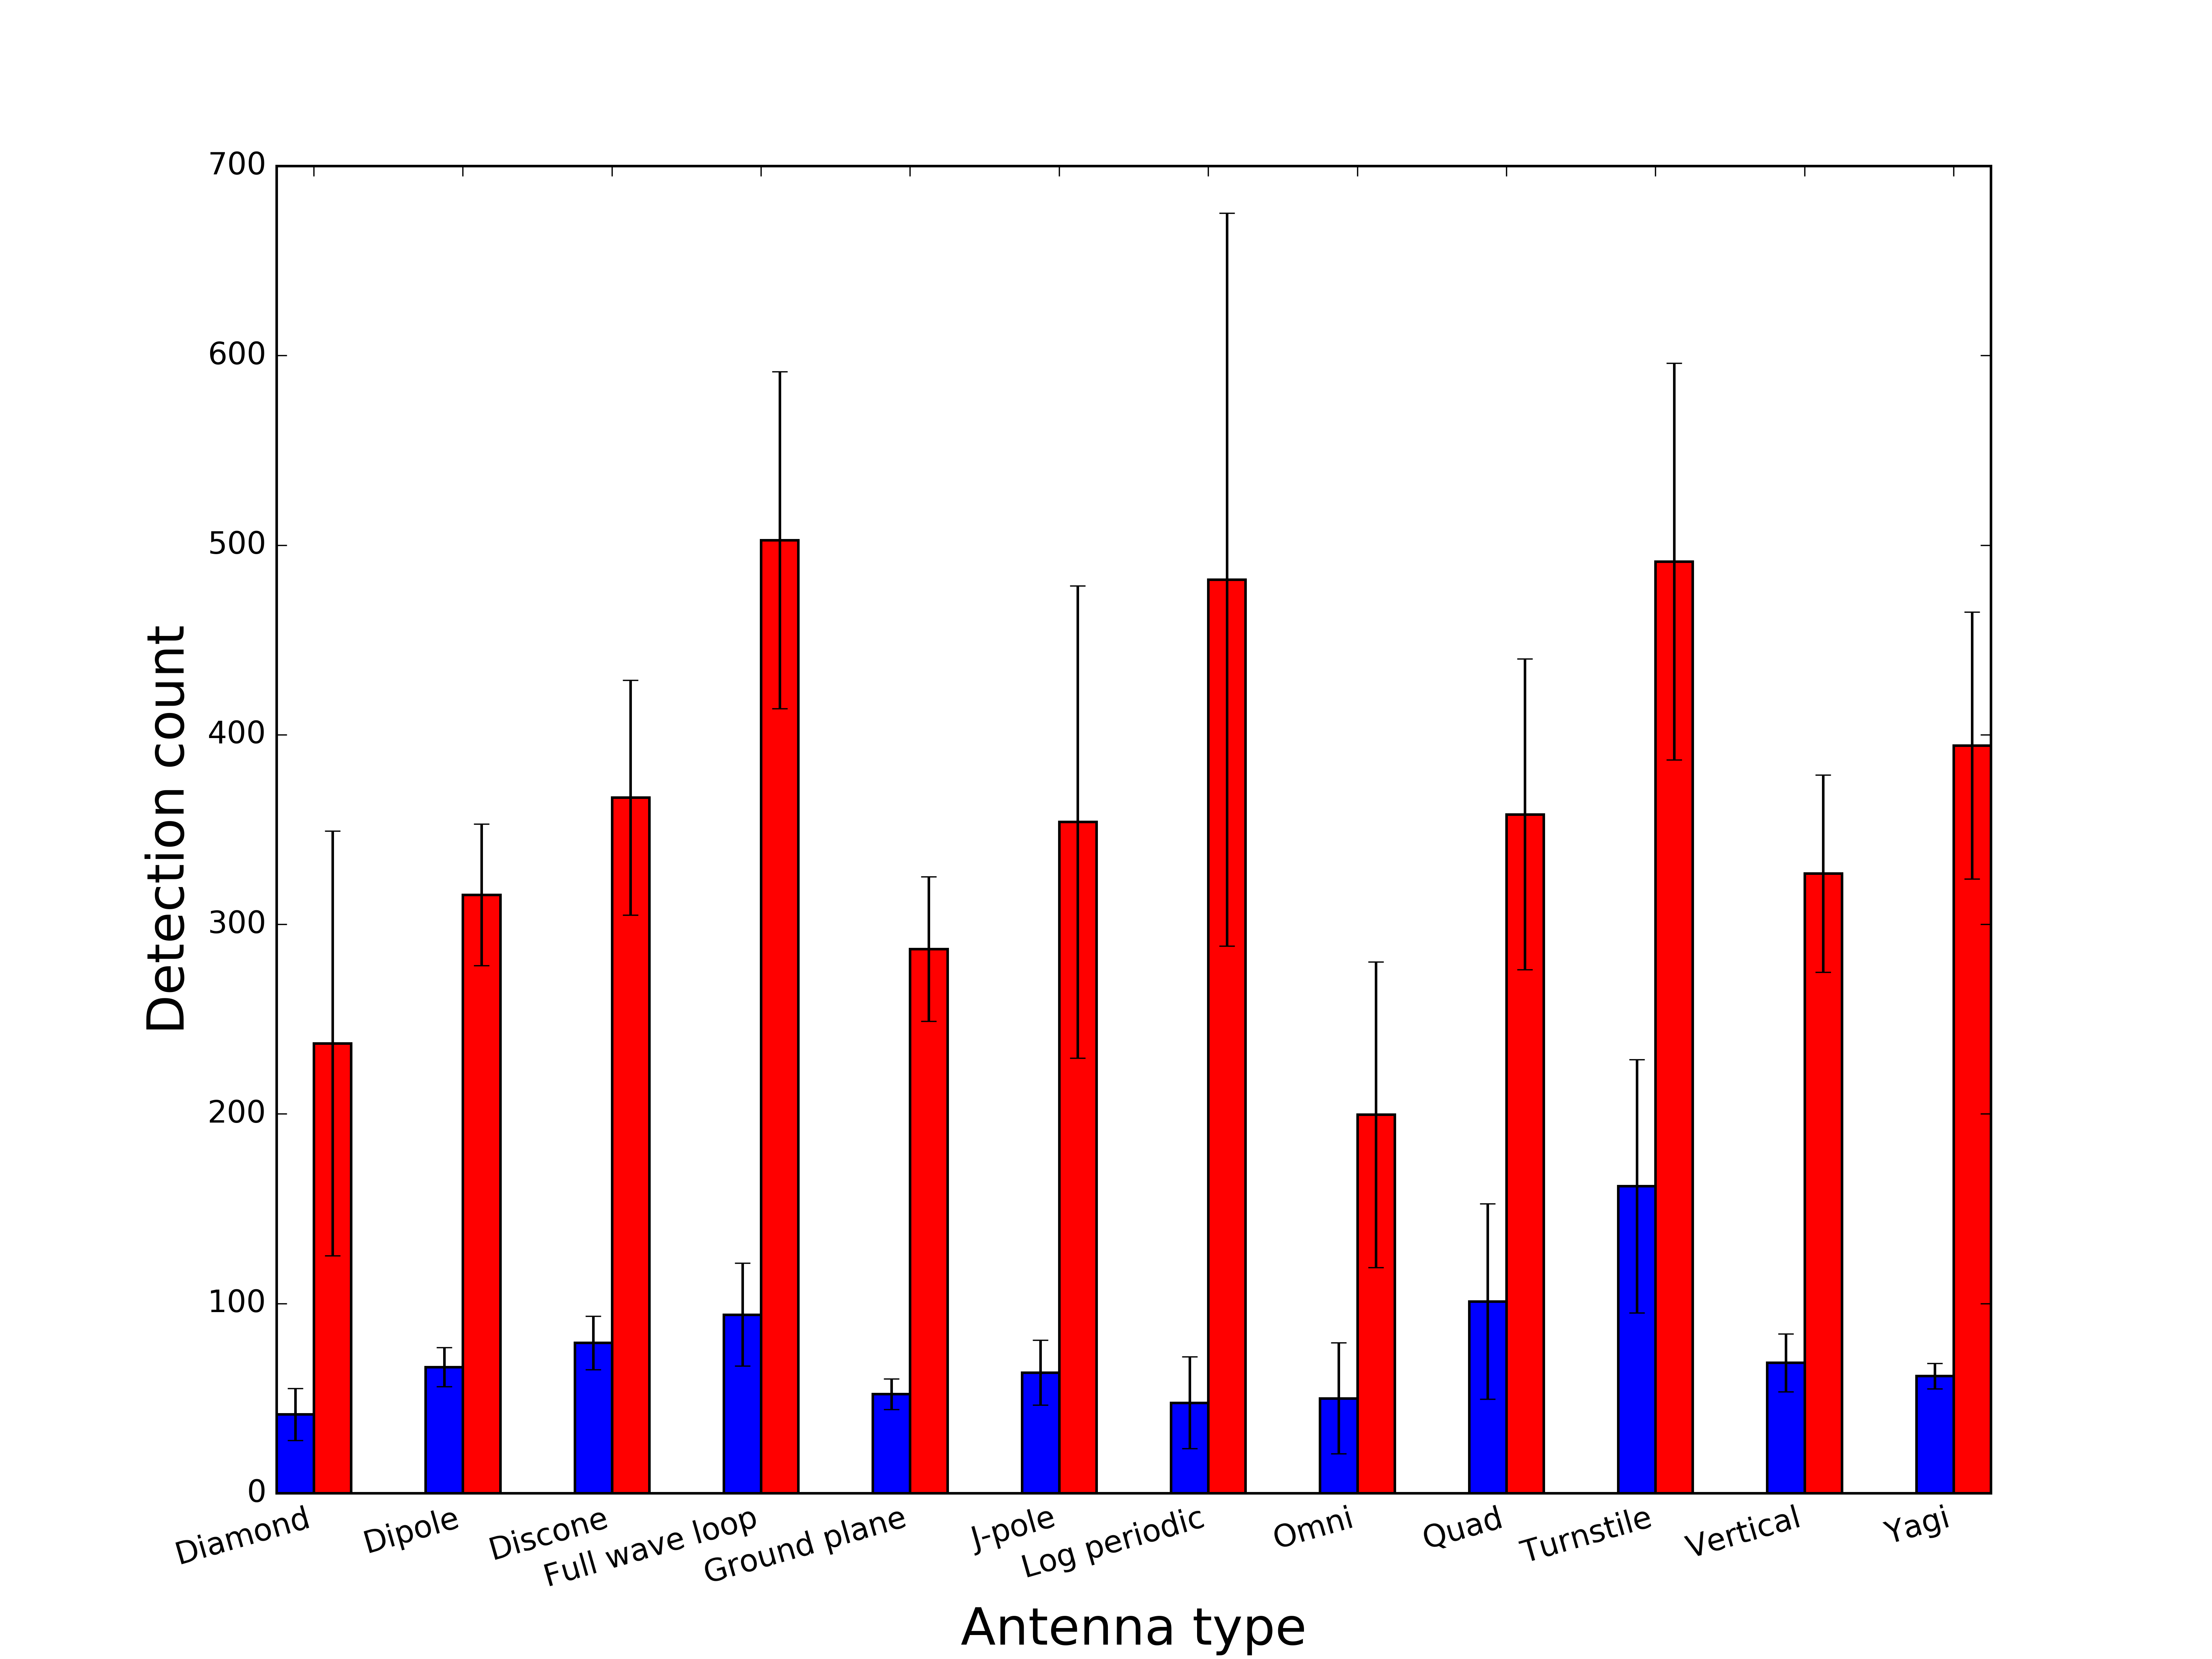
\includegraphics[width=\linewidth]{antenna/meanmaxmin}
	\caption{Mean and maximum hourly detection counts (maximum count in red, mean in blue)
		\label{fig:ant:meanmaxmin}}
\end{figure}

\subsection{Standard error}
Figure~\ref{fig:ant:err} shows the results for the mean standard error of the hourly counts for each antenna category. The most extreme values have the largest error bars, suggesting that this is because there is a small sample size. However, the turnstile, vertical and j-pole antennas have the largest standard errors, suggesting these antennas produce data with the most variation. Log periodic, ground plane, full wave loop and diamond antennas have the 
lowest standard error suggesting the lower variation of the data.

\begin{figure}[h!]
	\centering
	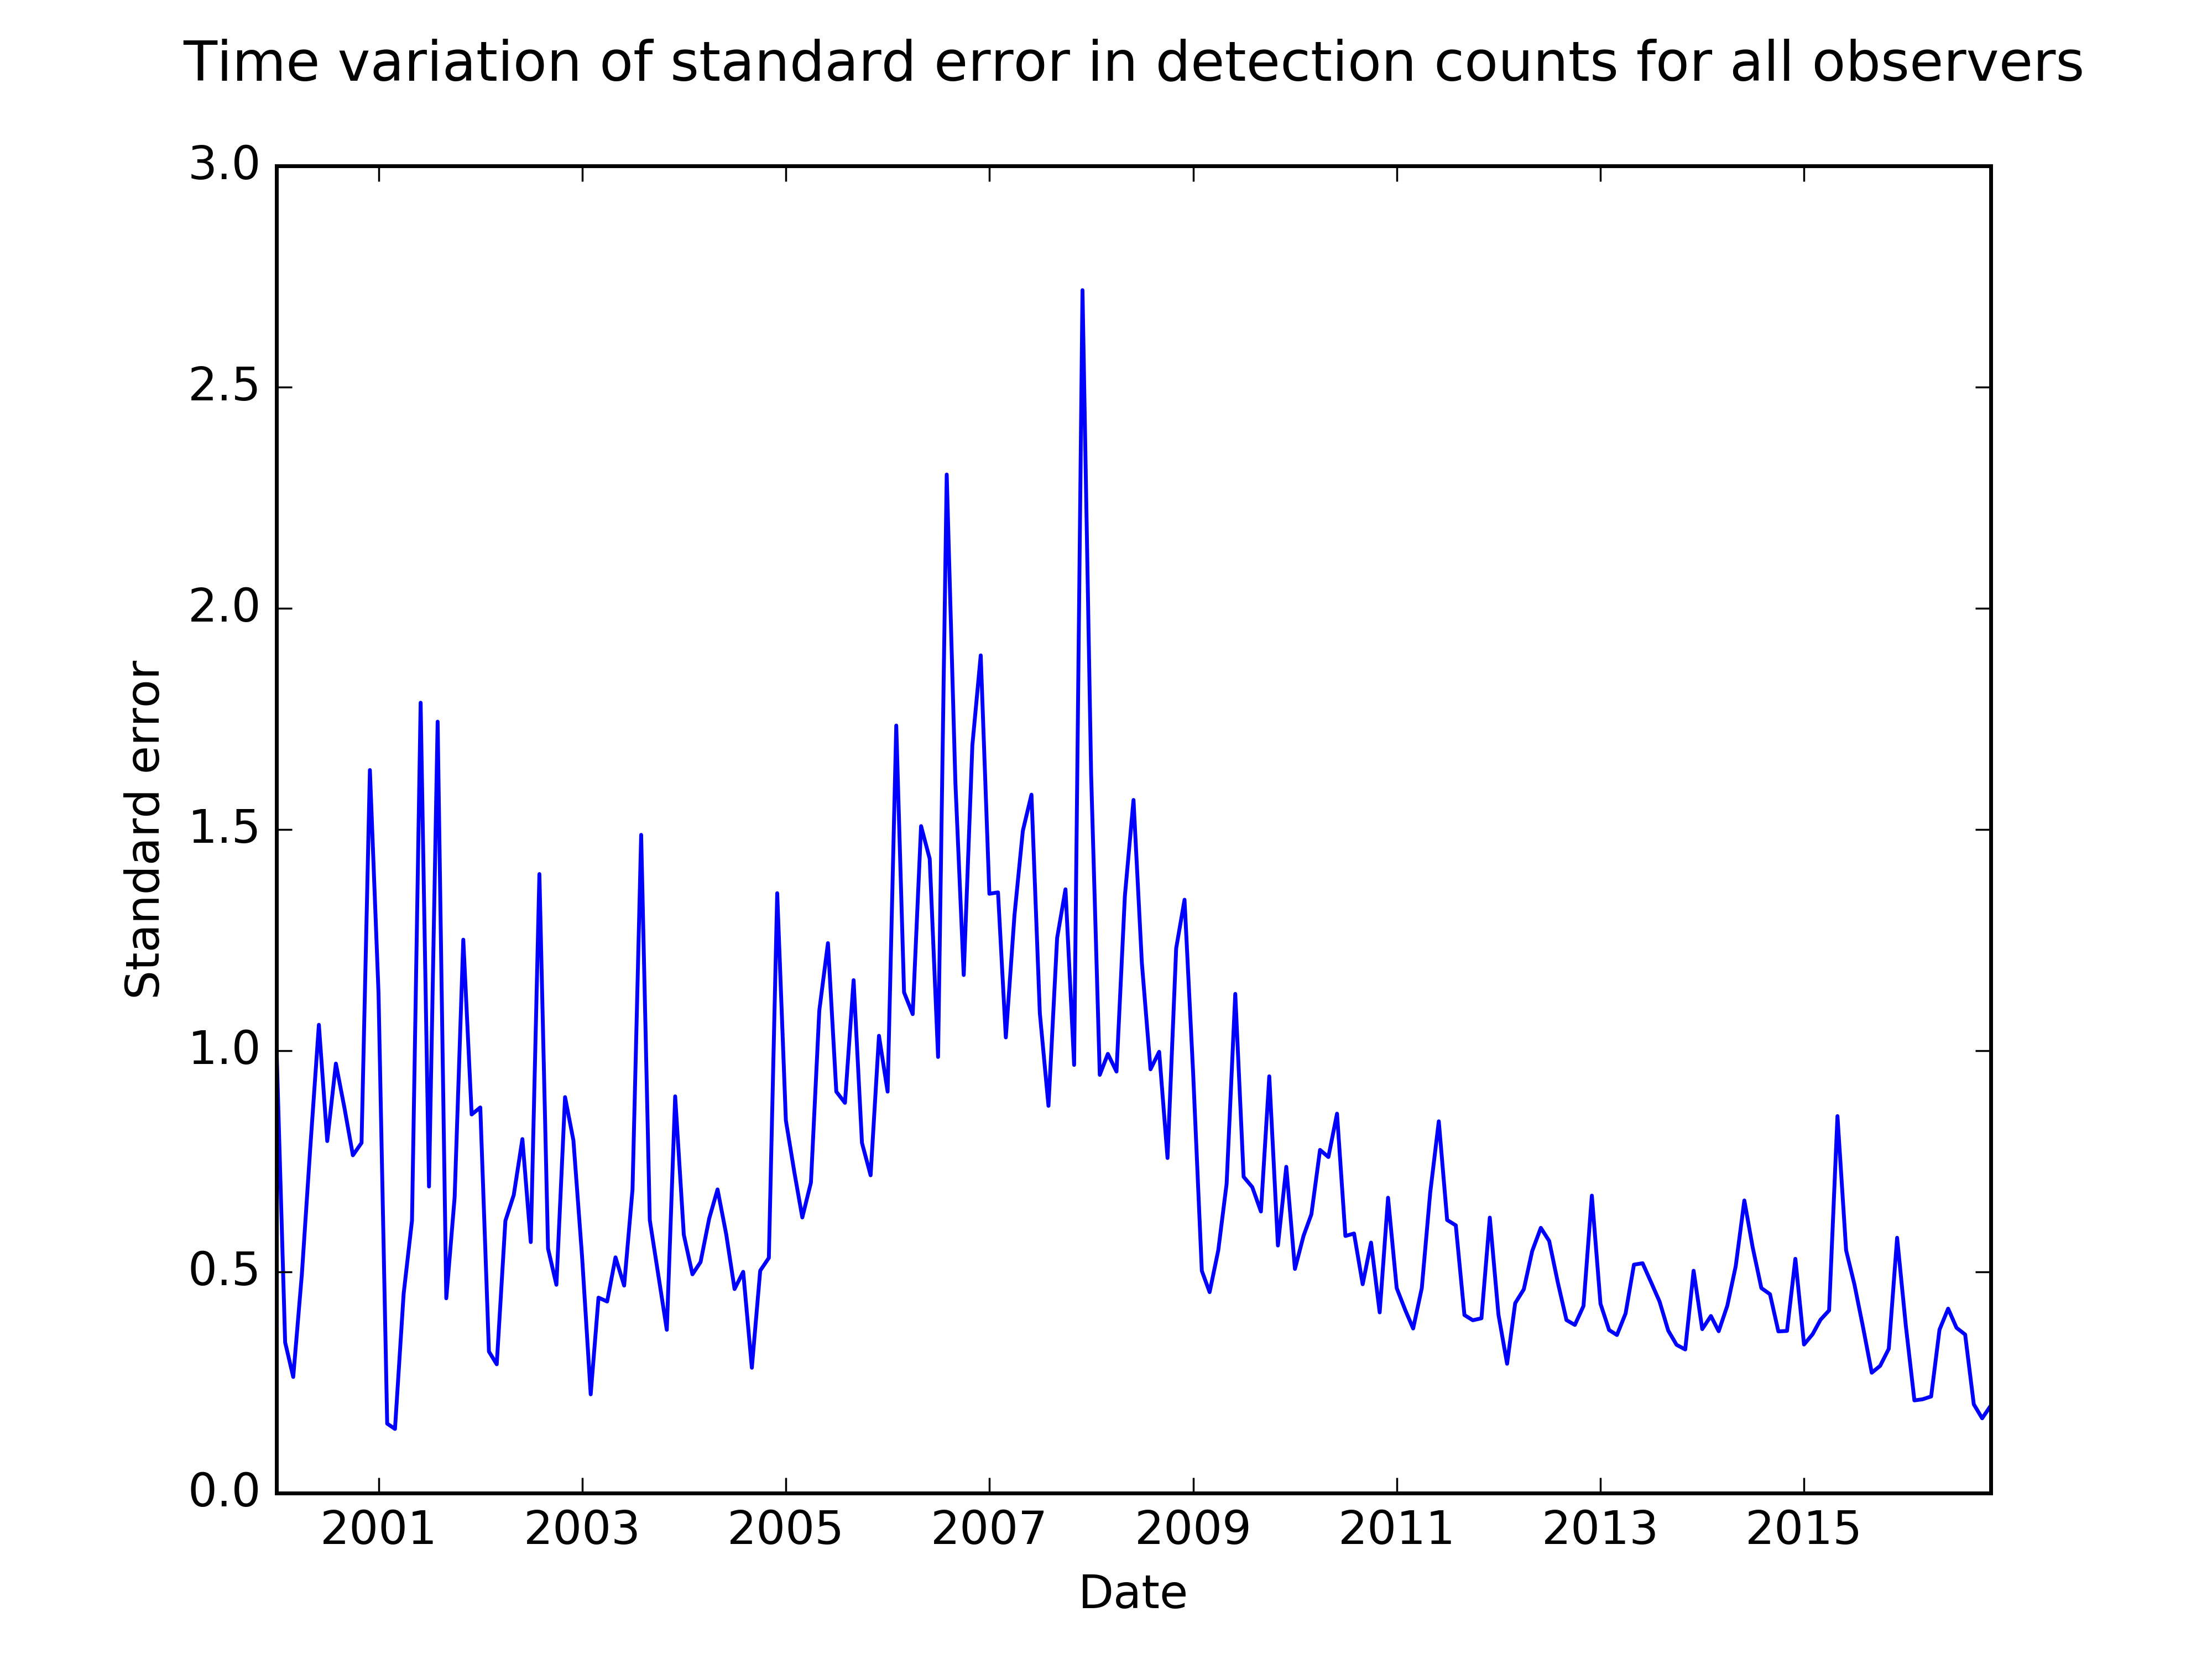
\includegraphics[width=\linewidth]{antenna/err}
	\caption{Variation of hourly detection counts
		\label{fig:ant:err}}
\end{figure}

\subsection{Skew}
From figure~\ref{fig:ant:skew}, it can be seen that log periodic, vertical and Yagi antennas have the largest positive skew, with turnstile, discone and full wave loop antennas with the largest negative skew. Generally, a positive skew is expected since the data should trail off towards larger counts, whereas no counts are valid below 0, so there is a steeper end to the distribution of data. This is not seen in the data. The skewness values for each antenna category are relatively evenly distributed around 0. 5 of the categories have a standard error in the skew that is larger than the skew itself, suggesting that these values are not significant and cannot be considered completely valid.

\begin{figure}[h!]
	\centering
	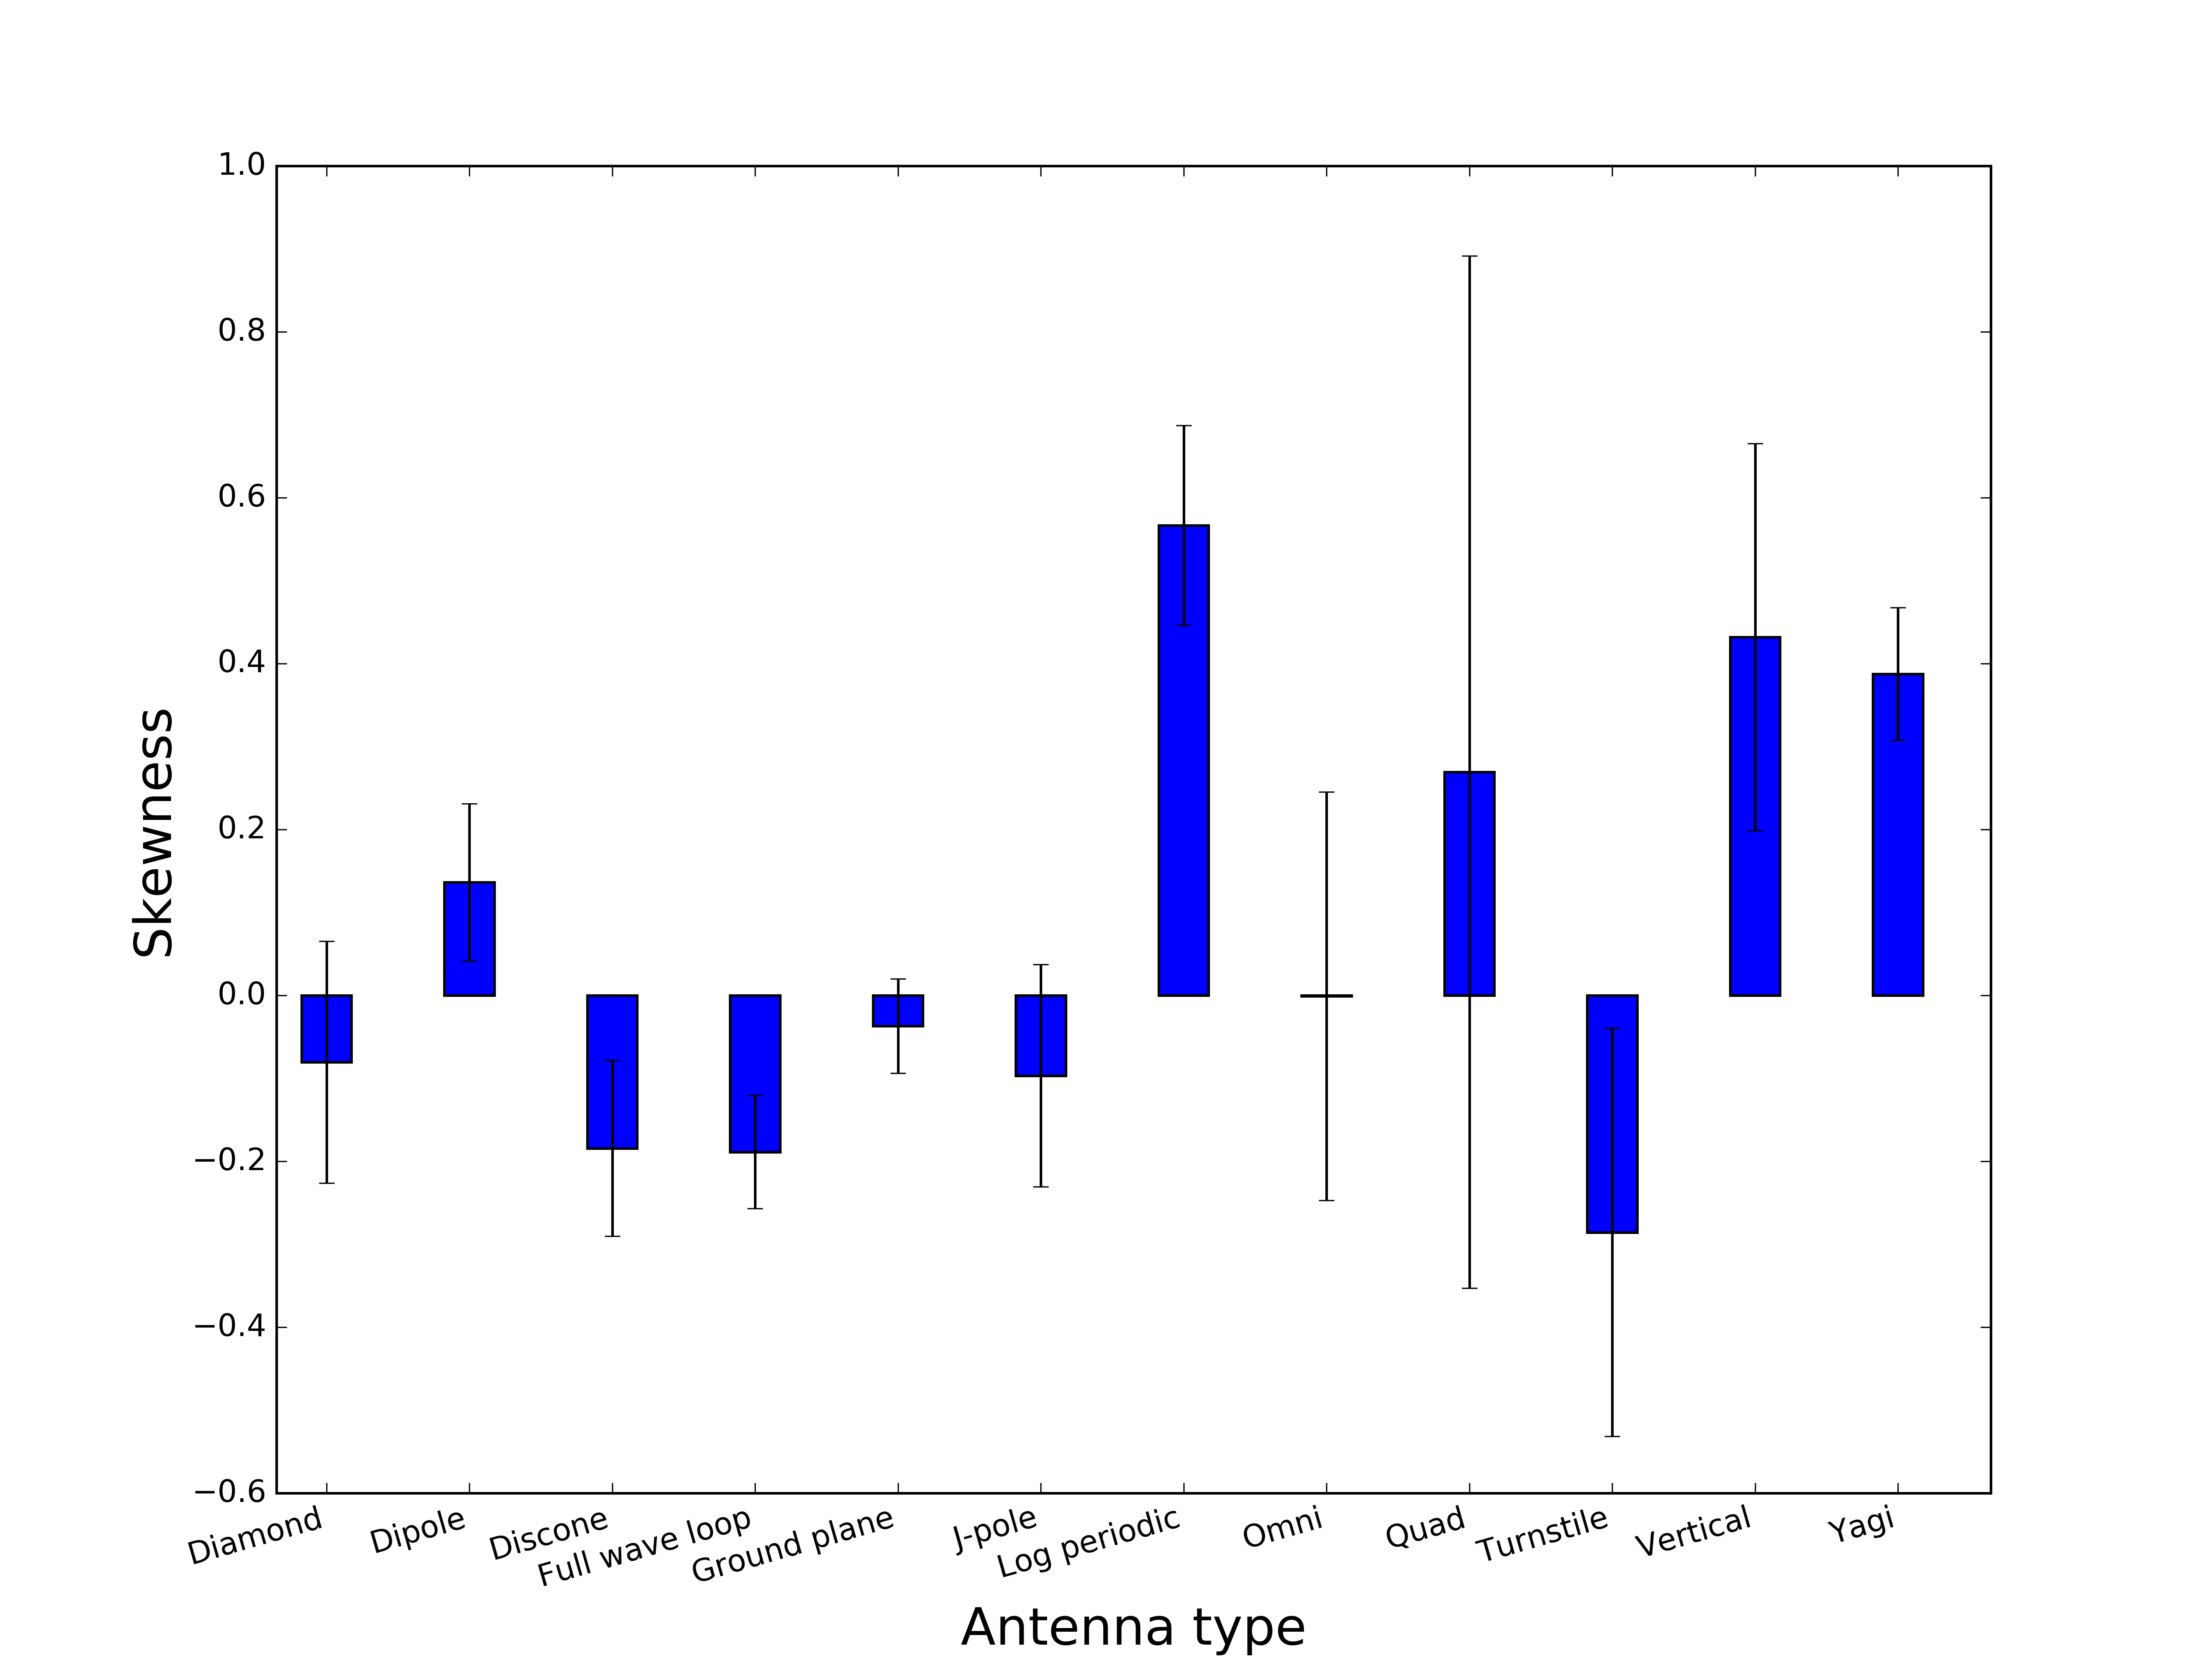
\includegraphics[width=\linewidth]{antenna/skew}
	\caption{Skewness of hourly detection counts
		\label{fig:ant:skew}}
\end{figure}

\subsection{Diurnal shift}
The results are relatively evenly distributed around a peak hour of 9: however, as found in chapter~\ref{chap:spatial}, this is most likely due to the geographical location where the antenna is used. Based on this, it is likely that ground plane, omni, quad and turnstile antennas are mostly used in Europe, whilst full wave loop, J-pole and diamond antennas are used mostly at latitudes ${\sim} -180^{\circ}$ and $180^{\circ}$.

\begin{figure}[h!]
	\centering
	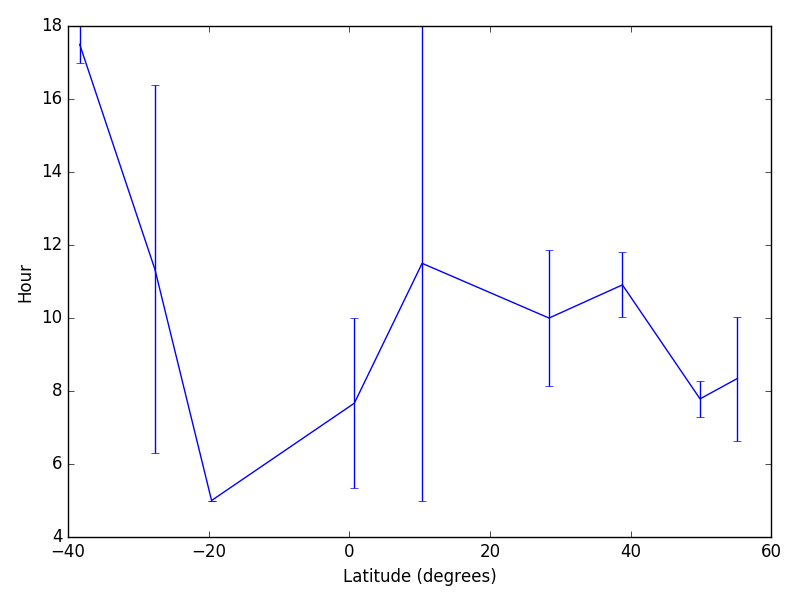
\includegraphics[width=\linewidth]{antenna/peak}
	\caption{Peak hour of diurnal shift
		\label{fig:ant:peak}}
\end{figure}

The larger results for J-pole, quad, turnstile and vertical antennas suggests that these are not as influenced by diurnal shift. However, these categories have much larger standard errors than other categories, suggesting that there is simply a low sample size. Vice versa, ground plane and log periodic antennas have much better fits to a sine curve, implying the antennas are more influenced by diurnal shift.
\begin{figure}[h!]
	\centering
	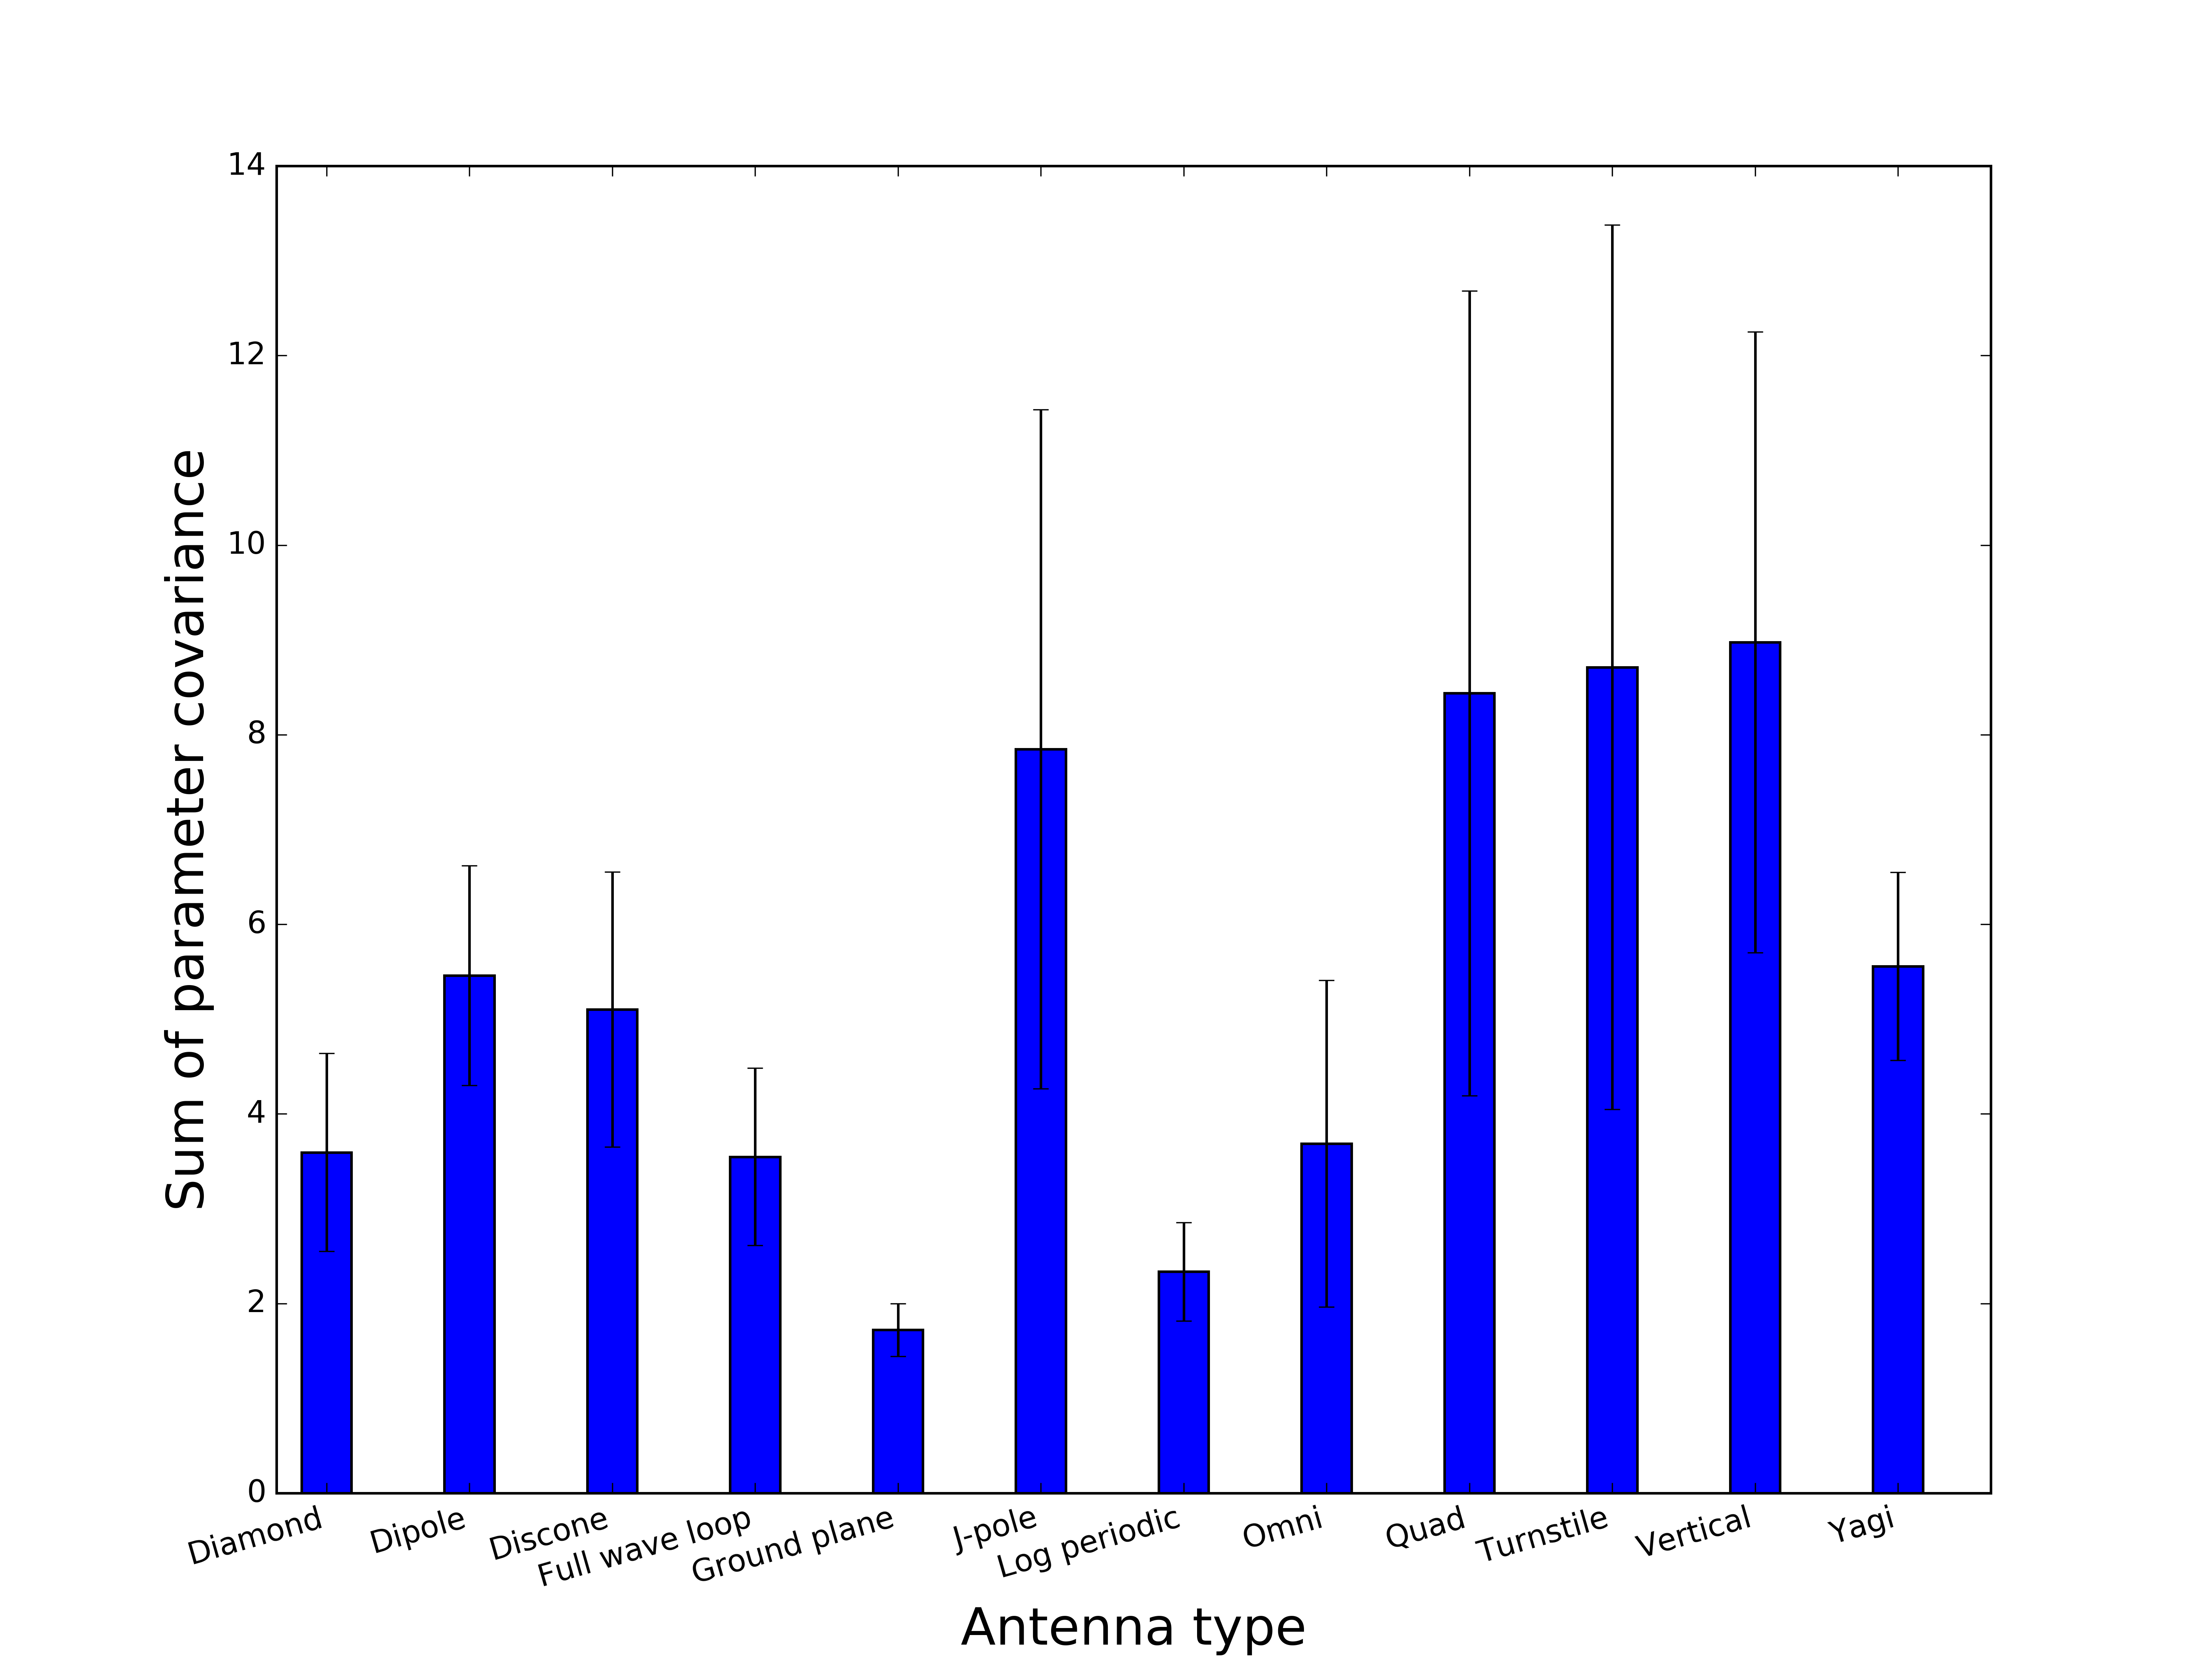
\includegraphics[width=\linewidth]{antenna/fit}
	\caption{Fit to optimal sine function for diurnal shift
		\label{fig:ant:fit}}
\end{figure}

\section{Discussion}
\subsection{Mean \& maximum}
There is no clear trend for an antenna which produces data which, on average, has greater hourly counts. This is expected. Were there an antenna that was particularly good at radio meteor detection, it would likely be used widely. Equally, if there was an antenna that produced particularly poor data, it would not be used at all. The standard errors, for all categories, range across ${\sim}$ 20 counts an hour. This is substantial, and suggests that there is little agreement between characteristics of data for observers that use the same antennas.
\subsection{Standard error}
For some categories, the mean standard error is much larger. However, these categories have greater errors. Diamond, full wave loop, ground plane, and log periodic antennas appear to produce data with the lowest amount of variation. The implication is that the antennas are poor at detection meteors, so there will be little variation in the counts. However, comparing these categories with figure~\ref{fig:ant:meanmaxmin}, they are the lowest categories (other than full wave loop), but not significantly lower than others. 
\subsection{Skew}
Log periodic, vertical and Yagi antennas all appear to produce reasonably positively skewed data. The same extremity is not seen for a negative skew. Other than vertical antennas, the error is not too large, indicating that there is {\it some} correlation. A lack of correlation with other properties indicates that this is an anomalous result. However, further investigation may yield this to be false.
\subsection{Diurnal shift}
Variations in the peak hour of diurnal shift are likely due to location, as discussed in chapter~\ref{chap:diurnalshift} and \ref{chap:spatial}. However, most antennas appear to produce data with peaks around hour ${\sim}$ 9. Errors for all categories are substantial, indicating little agreement within each category. Ground plane and log periodic antennas appear to produce data that fits a sine-function very well, indicating a greater periodicity in the data than other antennas. The poorest fits have large standard errors, indicating that these values are of little validity.
\subsection{Improvements}
\paragraph{Location}
From previous chapters, it is known that the location where data is collected will influence the results. Because of this, simply grouping together observers who use the same antenna may not give an accurate reflection of the data characteristics unless the data is somehow normalised so that location has no effect. The simplest way to do this is to include more observers, and then analyse the antenna categories. When comparing these results, the location can be factored into any conclusions, removing the influence that location has on the data.
\paragraph{Yagi n-element analysis\\}
In my analysis I have grouped {\it all} Yagi antennas into the same category. An analysis based on the number of elements on the antenna within the yagi category may indicate if there is an optimal number of elements for meteor detection, as well as the effect of different numbers of elements on the characteristics of the data.
\paragraph{Coefficient of variation\\} 
Instead of using standard error of the hourly detection counts to indicate the variation of the data, it may be better to use the coefficient of variation, $c_v$, defined as $c_v = \frac{\sigma}{\mu}$ where $\mu$ and $\sigma$ are the mean and standard deviation of the data respectively. This gives a better reflection of the variation as instead of factoring in the sample size, it factors in the mean. This is an improvement since the degree of variation is no longer proportional to the mean, giving no skew favouring lower means.
\paragraph{Percentiles\\}
As part of the data characteristics analysis, I used the maximum count to help summarise the data. This is not a very useful summary value to make, since the maximum itself holds little value. What would indicate the distribution of data better is a value such as the 90th percentile. This may give a better reflection of the data that an antenna produces.
\section{Conclusion}
There is no clear correlation between any characteristics and the antenna types. However, J-pole, log periodic and turnstile antennas consistently have the most extreme values. However, the extremes for these antenna types do not necessarily imply the same characteristics of the data. Log periodic antennas appear to provide consistently positive-skewed data. Turnstile antennas appear to provide the largest detection counts. A consistent theme throughout the results are large errors, suggesting large variation within each antenna category, implying little correlation between the given antenna type and the characteristic under consideration. Greater sample sizes, as well as isolation of other variables (location, time) may reveal more correlation.